\chapter{Results}
The results have been summarized in the following sections and the code files are also provided specific to each section.

\section{GB effects in a two-grain system}
In this Figure we show the evolution of microstructure in a two-grain system (with periodic boundary conditions along both x and y axes) in system \textbf{Ia}(a defined earlier) for \textbf{t=10, 50 and 200}, for an alloy of composition $\mathbold{c_o = 0.5}$ and with initial fluctuations of $\mathbold{\delta_c = 0.04}$. For this system, $\mathbold{\gamma_\alpha}$, the $\mathbold{\alpha}$-GB energy is about 18\% lower than $\mathbold{\gamma_\beta}$. This difference provides the driving force, during early stages, for the GB to acquire species A.

This process of GB enrichment with species A also leads to the formation of a B-enriched layer (white band) followed by a faint A-rich band (dark grey) on either side of the boundary in the figure. During this time, the grain interior undergoes normal SD; the extent of this decomposition, however, is much smaller than that at the boundaries. At t = 50, the microstructure shows three bands at and near the GB in each grain (starting with the $\mathbold{\alpha}$ band at the GB, followed by a $\mathbold{\beta}$ band and a second $\mathbold{\alpha}$ band), coexisting with a grain interior exhibiting normal SD.
\begin{figure}[H]
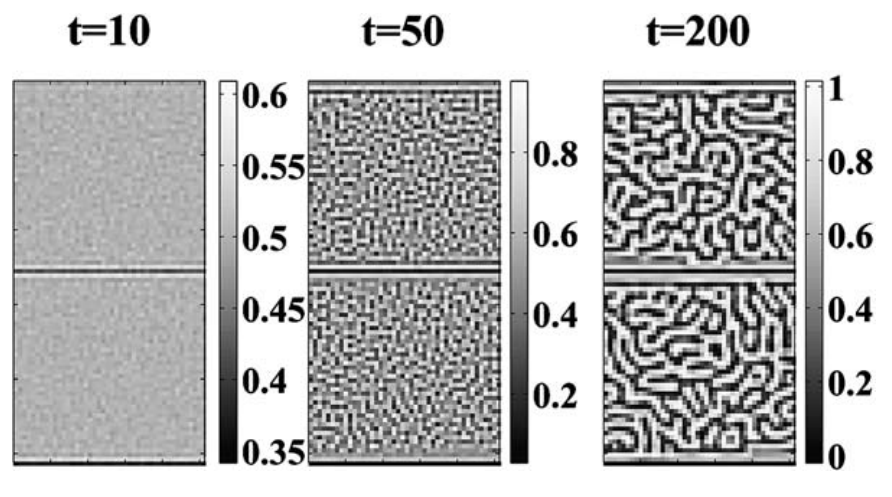
\includegraphics[width=\linewidth]{Fig2A}
\caption{Actual Figure}
\end{figure}

\begin{figure}[H]
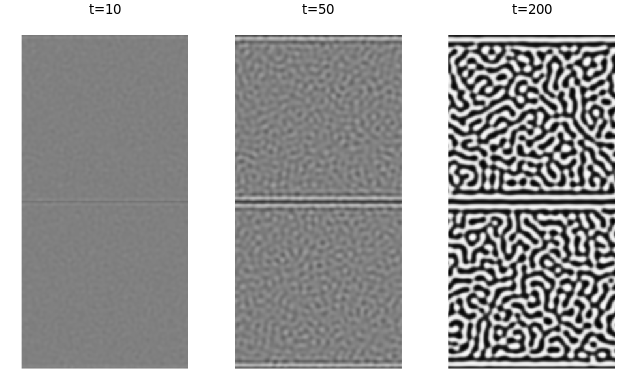
\includegraphics[width=\linewidth]{Fig2}
\caption{Reproduced Figure}
\end{figure}

\section{Effect of ($\mathbold{\gamma_\beta-\gamma_\alpha}$) and initial fluctuation}
The microstructural evolution depicted in the above figure may be described in terms of a competition
between two different phenomena: 
\begin{enumerate}
\item GB assisted phase separation which initiates a composition wave which travels into the grains and is faster than the other
\item normal SD in the grain interior which leads to the formation of a bicontinuous microstructure of A-rich and B-rich regions
\end{enumerate}

From the results(as shown in figure) we may infer that the number of bands near the GB would be 
\begin{enumerate}
\item higher if the normal SD in grain interiors can be delayed (e.g., by using smaller fluctuations (noise) in the initial configuration), and  
\item lower if the driving force (gamma|beta-gamma|alpha) for the GB enrichment with species A is made smaller. \end{enumerate}

We test these hypothesis in this section\\
We compare the following 3 systems at t=100
\begin{enumerate}

\item System Ia @ $\mathbold{\delta_c = 0.04}$; this represents a high driving force for the GB enrichment, and high initial noise. It shows three bands in each grain.
\item System Ia @ $\mathbold{\delta_c = 0.01}$; similar to the later case but with a lower initial noise which delays normal SD and allows for GB assisted phase separation. It shows 5 bands.
\item System IIa @ $\mathbold{\delta_c = 0.01}$; Same lower initial noise together with further reduced driving force which reduces the GB assisted phase separation compared to the previous phase and so we only see 4 bands.

\end{enumerate}

\begin{figure}[H]
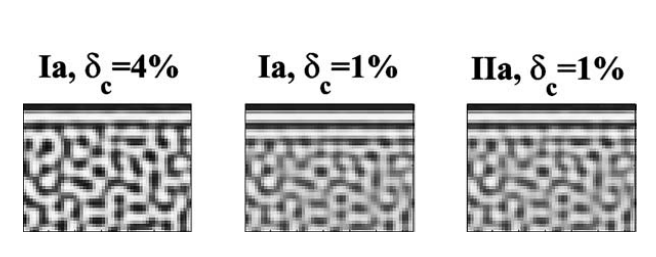
\includegraphics[width=\linewidth]{Fig3A}
\caption{Actual Figure}
\end{figure}

\begin{figure}[H]
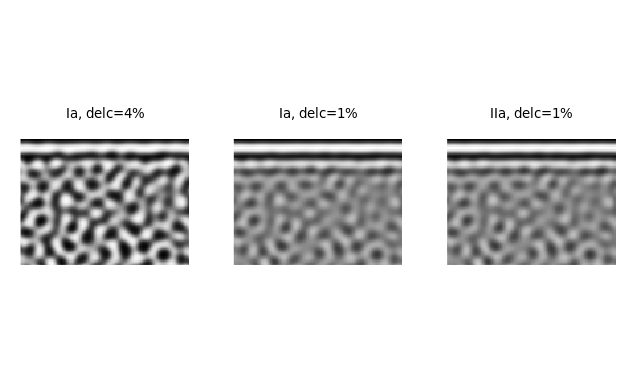
\includegraphics[width=\linewidth]{Fig3}
\caption{Reproduced Figure}
\end{figure}

\subsection{Analysis of deviation of composition from average composition with distance from the GB}
The difference $\mathbold{c_p-c_o}$ as a function of distance from the GB, where $\mathbold{c_p}$ is the average composition within a layer parallel to the GB and $\mathbold{c_o}$ is the alloy composition. The figure below shows that the composition wave is initiated at the GB, and propagates into the grain interiors; further, for a given time, this composition wave also decays with distance from the GB.

\begin{figure}[H]
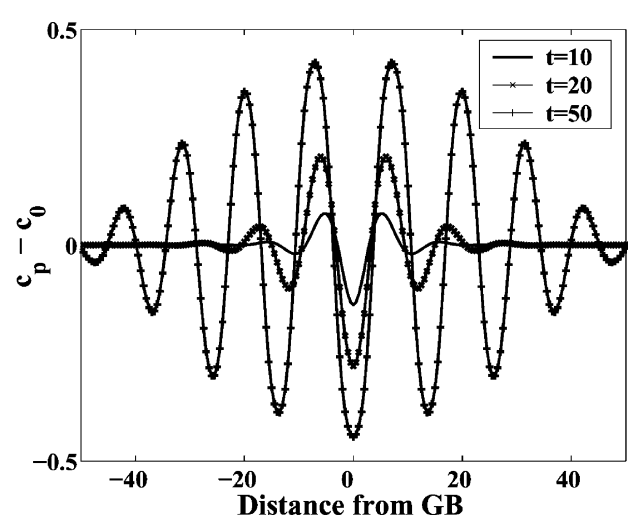
\includegraphics[width=\linewidth]{Fig4A}
\caption{Actual Figure}
\end{figure}

\begin{figure}[H]
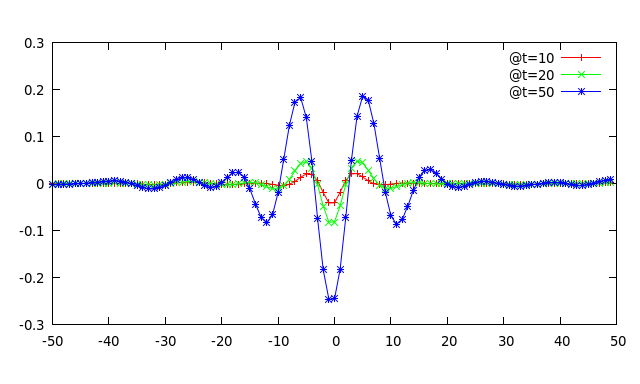
\includegraphics[width=\linewidth]{Fig4}
\caption{Reproduced Figure}
\end{figure}

\subsection{$R_1$(t) vs t}

$\mathbold{R_1(t)}$, the first zero of the $\mathbold{c_p-c_o}$ profile, is plotted as a function of time for systems Ia, lb and Ic. It is clear that $\mathbold{R_1}$ increases with time, before stabilizing towards late stages. More importantly, the $\mathbold{R_1(t)}$ behaviour is essentially the same in these three systems, indicating that differences in GB widths (in system Ic) or in incoherent boundary energy (in system Ib) do not play a significant role in determining the formation of GB-bands.

\begin{figure}[H]
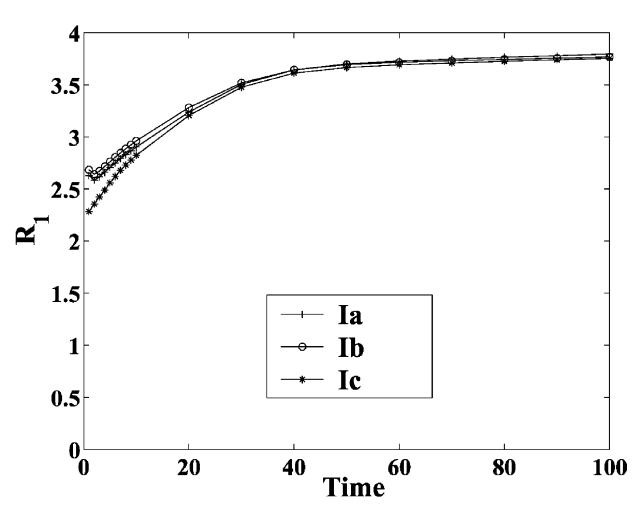
\includegraphics[width=\linewidth]{Fig5A}
\caption{Actual Figure}
\end{figure}

\begin{figure}[H]
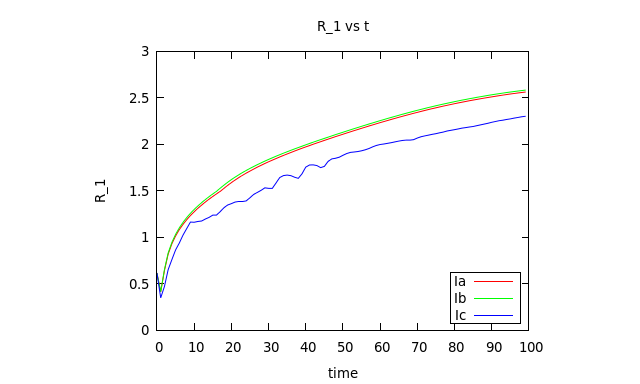
\includegraphics[width=\linewidth]{Fig5}
\caption{Reproduced Figure}
\end{figure}

\section{Number of GB bands}
A different analysis of the GB-initiated composition wave can be used for estimating the number of GB bands in the microstructure. This analysis is based on the extent of decomposition defined by:

\begin{equation}
f_D=\frac{\int_{V_b} (c_p-c_o)^2 dV}{V_b c_o (1-c_o))} 
\end{equation}

where $\mathbold{V_b}$ is the volume of interest,
By definition, $\mathbold{f_D=0}$ for a homogeneous alloy, and $\mathbold{f_D=1}$ at equilibrium.
The hypothesis we wish to test is that the GB initiated composition wave (and the associated band formation) progresses into the grain until it encounters a region that has decomposed to a significant extent. For this purpose, $\mathbold{f_D}$ is estimated separately for each of the bands in a simulation of GB-assisted SD, which is carried out with no initial composition fluctuation within the grains. 
These $\mathbold{f_D}$ values for individual bands are plotted as a function of time, and compared with similar plots for two bulk simulations (with no GB) of system Ia starting with an initial noise of $\mathbold{\delta_c = 0.04}$ and $\mathbold{\delta_c = 0.01}$.
From the figure the curve for the fourth band lies close to that for the bulk simulation with a higher initial noise $\mathbold{\delta_c = 0.04}$. This implies that a fourth band is unlikely to form in this system. Fig. \label{3A} ($1^{st}$ part) shows that this is indeed the case.
In a similar way, since fD curve for the sixth band is close to that for the bulk system with $\mathbold{\delta_c = 0.01}$, we may expect only five bands for this system. again, Fig. \label{3A} ($2^{nd}$ part) shows that this is indeed the case.

\begin{figure}[H]
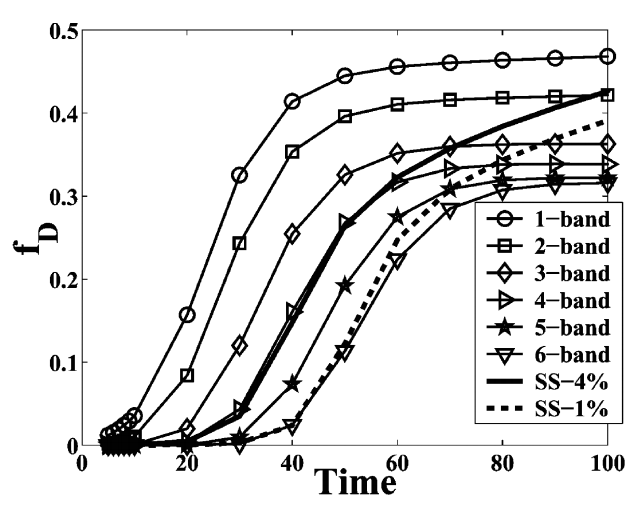
\includegraphics[width=\linewidth]{Fig6A}
\caption{Actual Figure}
\end{figure}

\begin{figure}[H]
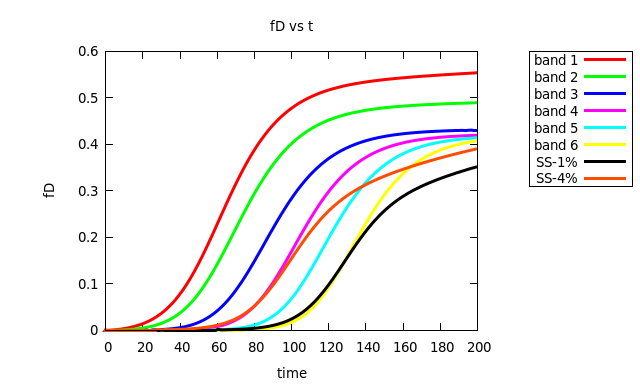
\includegraphics[width=\linewidth]{Fig6}
\caption{Reproduced Figure}
\end{figure}



